\documentclass[10pt,a4paper,book,openany]{jlreq}

\usepackage{graphicx}
\usepackage[pdfencoding=auto]{hyperref}
\usepackage{amsmath,amssymb,amsthm}
\usepackage{bm}
\usepackage{booktabs}
%\usepackage{subfig}
\usepackage{pifont}
\usepackage{url}
\usepackage{cite}
\usepackage{ulem}
\usepackage{siunitx}
%\usepackage{physics}
\usepackage{float}
\usepackage{tcolorbox}
\tcbuselibrary{breakable}
\usepackage{cancel}
\usepackage{color}
\renewcommand{\CancelColor}{\color{red}}

\theoremstyle{definition}
\newtheorem{theorem}{定理}[chapter]
\newtheorem*{theorem*}{定理}
\newtheorem{definition}[theorem]{定義}
\newtheorem*{definition*}{定義}

\usepackage{xcolor}
\hypersetup{
  bookmarksnumbered=true,
  colorlinks=true,
  citecolor=red,
  linkcolor=blue,
  urlcolor=orange,
}

\begin{document}
\title{SuperKEKBクライストロン電源}
\author{Shin-ichi YOSHIMOTO}
\maketitle
\tableofcontents
\clearpage

%\part{something}

\chapter{クライストロン電源の概要}

\section{RFシステムの概要}

SuperKEKB加速器は4つの直線部を4つの弧で結んだレーストラック型で、4つの直線部のうち3箇所と陽電子用のダンピングリングに電子や陽電子を加速するための高周波システムが配置されています。(残りの直線部にはBelle II測定器があります)図\ref{layout}にSuperKEKB加速器の高周波システムのレイアウトを示します。大穂(D4, D5)、富士(D7, D8)、日光(D10, D11)、ダンピングリングの四つの電源室に、電源1台で2本のクライストロンに電力を供給できるA型電源14台、電源1台で1本のクライストロンに電力を供給できるB型電源3台、計17台の電源設備があり、クライストロンは31本あります。電源装置は、できるだけ安価で安定した電源供給を目指したもので、殆どの電源が改良や老朽化対策を行いながら、設置から40年近く使い続けています。

電源とクライストロンは地上の電源室にありますが、そこから地下11 mにある周長3 kmの加速器トンネル内に加速空洞が設置されています。大穂と富士では常伝導空洞であるARES空洞が、日光では超伝導空洞が使われており、クライストロンから伸びた長い導波管でこれらの加速空洞へと繋がり、クライストロンから出た高周波電力が供給され、電子や陽電子を加速します。


\begin{figure}[!htt]
    \begin{center}
        \includegraphics[width=\linewidth]{figs/SKEKB-RF.pdf}
        \caption{Layout of SuperKEKB, showing the locations of RF buildings and RF stations.}
        \label{layout}
    \end{center}
\end{figure}

\section{クライストロン電源の概要}

SuperKEKBのメインリング(MR)のクライストロン電源(KPS)には、2台のクライストロンに電源を供給するA型と、1台のクライストロンだけのB型が存在する。さらに、A型及びB型の半数は、交流\qty{6.6}{\kilo\volt}ラインの位相を\qty{15}{\degree}ずらしてあり、MRの電源室へ混在させて設置してある。これは、MRビームへのカソード電圧のリップルを通して影響、及び、逆に\qty{6.6}{\kilo\volt}ラインを通して中央変電所側への高次のノイズの発生等を考慮して行われた。つまり、カソード電圧は12相の全波整流でクローバ回路部にあるコンデンサーで平滑され、その半数は\qty{15}{\degree}位相がずれており、MR全体で見た場合大略、24相で整流されたものとみなせる見なせる。

電源は、各クライストロン1本につき、カソード、アノード/ヒータ、集東/補助集束コイルの電源から構成される 。A型電源では、カソード電圧は2本のクライ-ストロンで共通であるが、その他は独立に制御される。出力電圧はトランスの切替(無電圧時) によって、公称出力\qty{-50}{\kilo\volt}、\qty{-65}{\kilo\volt}、\qty{-80}{\kilo\volt}及び\qty{-90}{\kilo\volt}の内から1つ選択され、さらに微細な電圧調整は、可変範囲$\pm \qty{10}{\percent}$のIVRによって行われる。実際の運転においてはクライストロン負荷が変化しても、$\Delta Vk/Vk<\pm \qty{1}{\percent}$となる様にIVRを自動転している。各クライストロンへはカソード電庄\qty{-90}{\kilo\volt} でビーム電流\qty{20}{\ampere}まで供給可能である。アノード電源はコッククロフトワルトン型の電源で、カソード電位が基準電位なり、\qty{+80}{\kilo\volt}で\qty{10}{\milli\ampere}まで出力可能である。実際の運転においては、立下りを早めることが必要となり(後述)\qty{20}{\mega\ohm}の抵抗を外付けにクライストロンと並列にカソードとアノード間に挿入した。

\begin{figure}[!htt]
    \begin{center}
        \includegraphics[width=\linewidth]{figs/skeleton-diagram.pdf}
        \caption{Block diagram of a type-A KPS.}
        \label{f02-02}
    \end{center}
\end{figure}

\begin{figure}[!htt]
    \begin{center}
        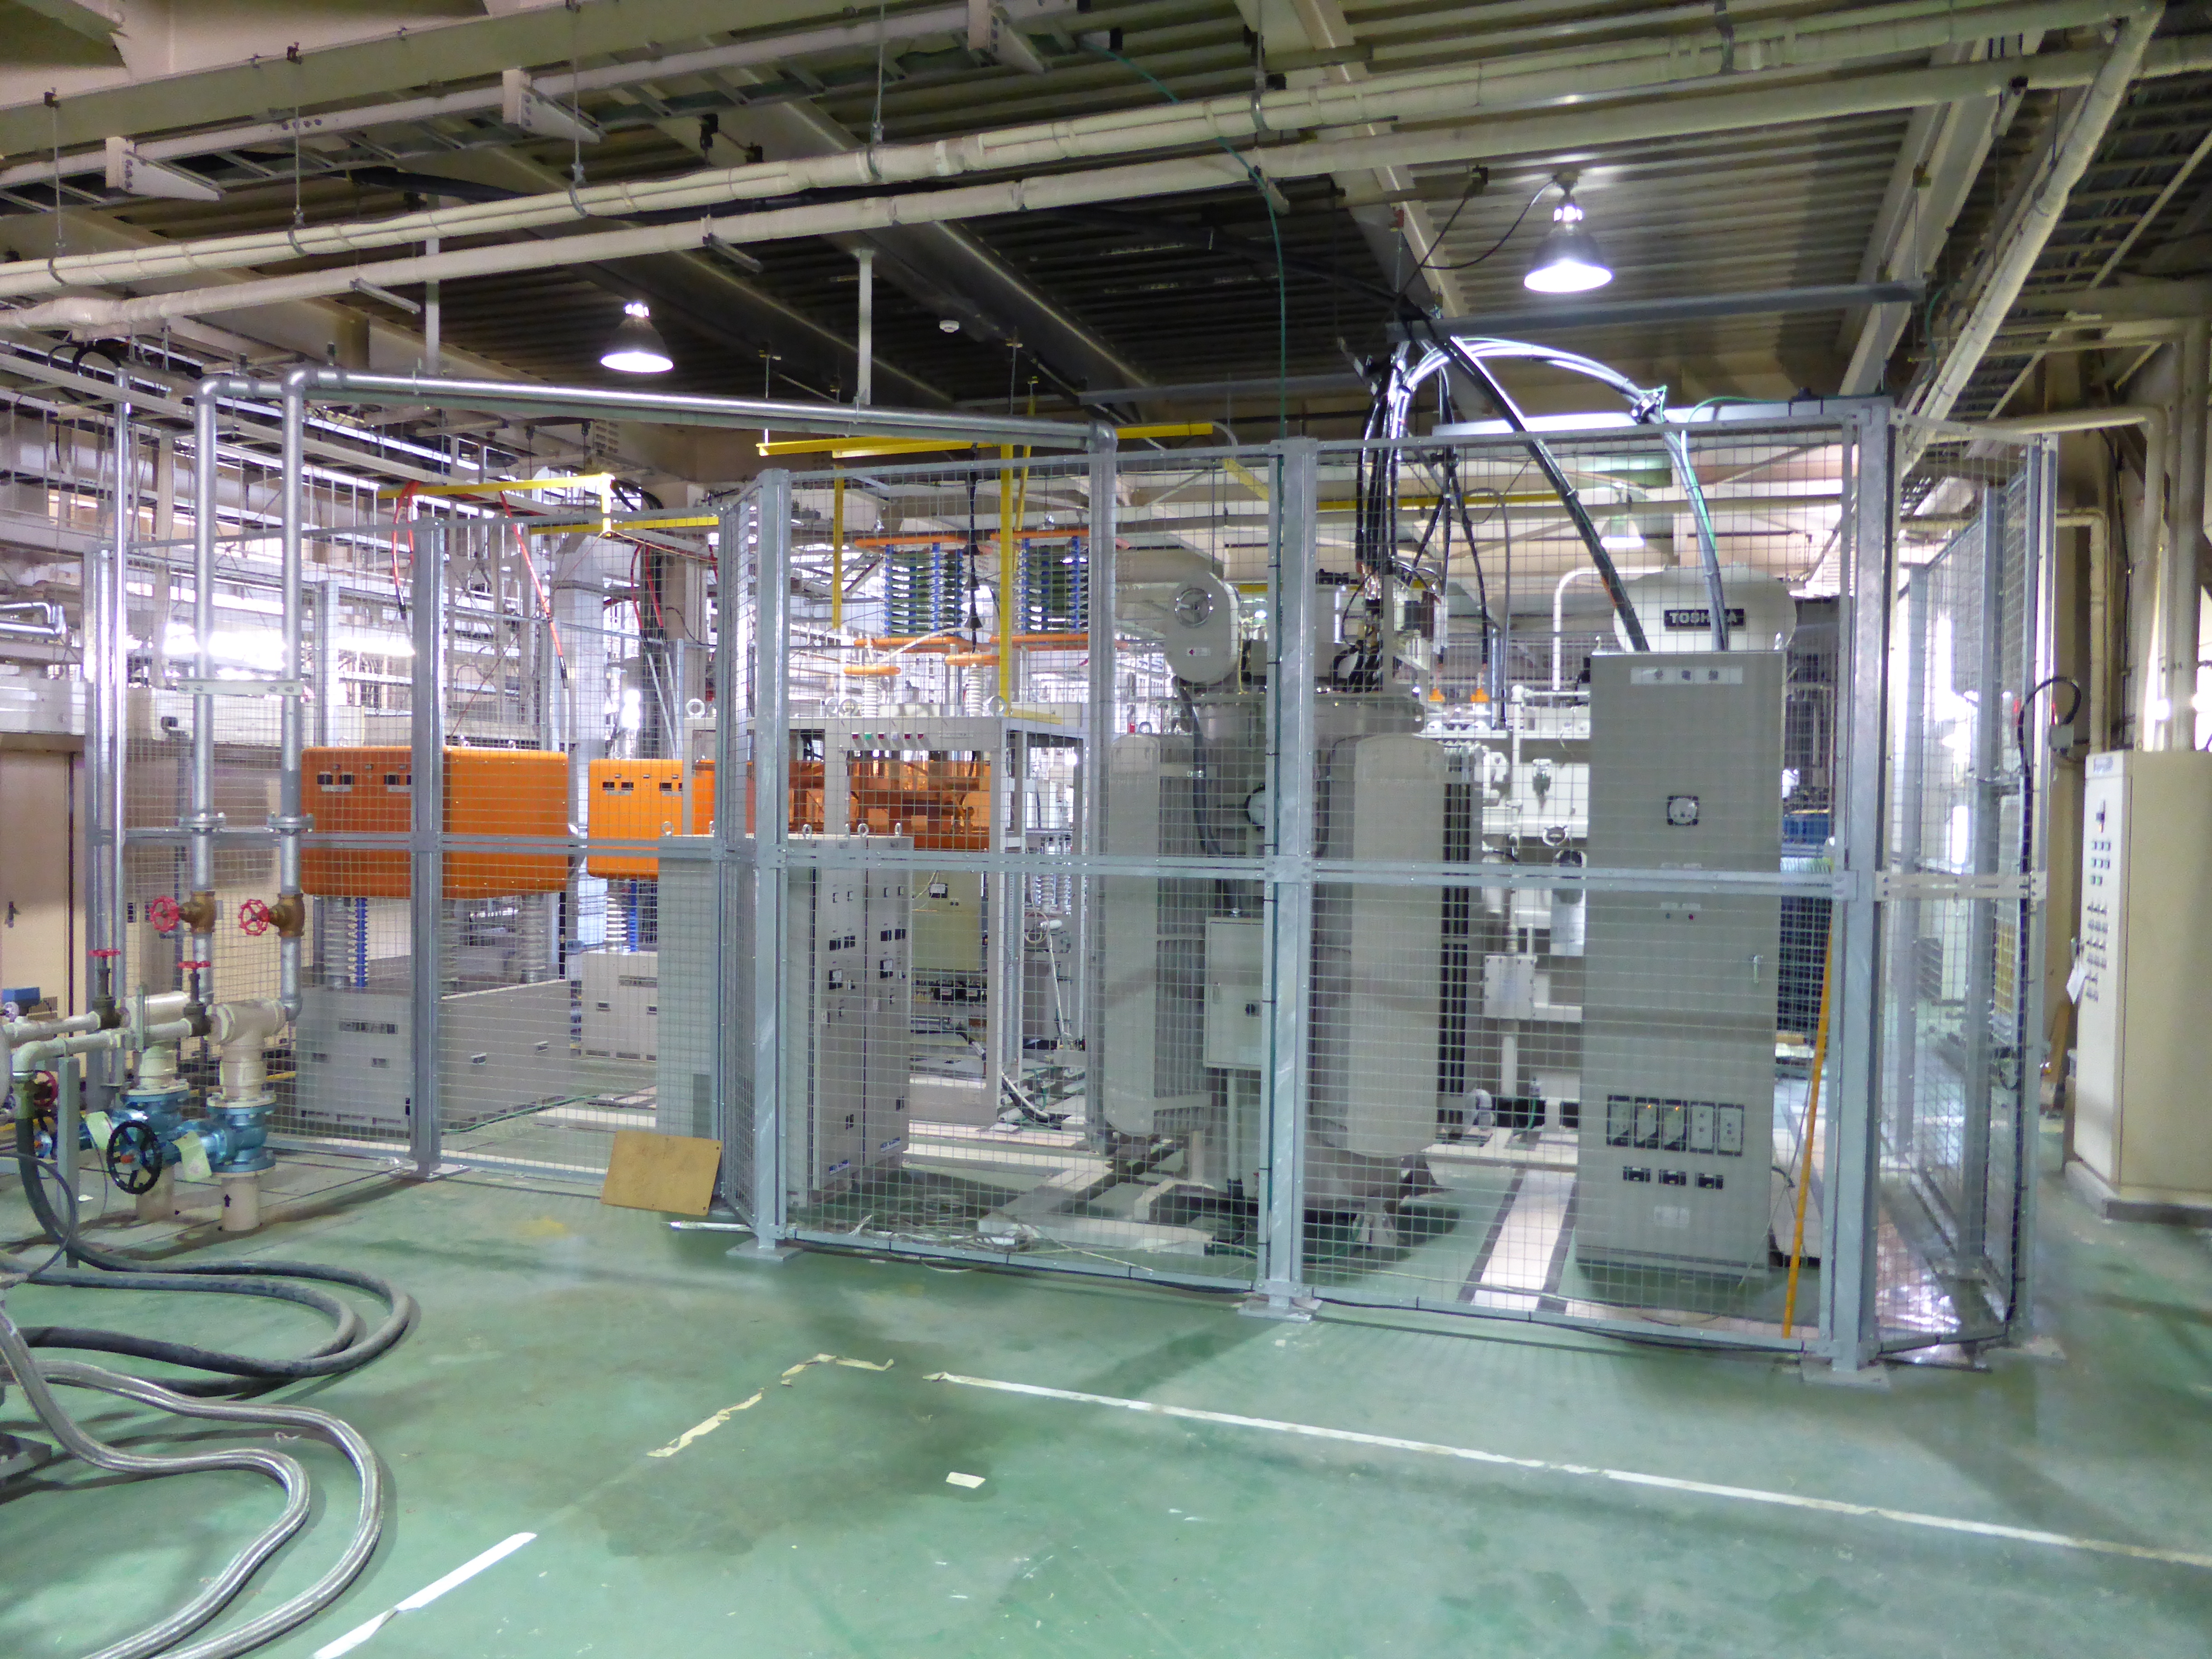
\includegraphics[width=\linewidth]{figs/KPS.JPG}
        \caption{クライストロン電源の全景}
        \label{kps_photo}
    \end{center}
\end{figure}

\subsection{直流高電圧カソード電源}
電源平滑コンデンサの容量を大きくすればするほど、リップル含有率は小さくなる。しかし、やみくもに大きくすれば良いという訳ではない。その理由は、電源投入時に平滑コンデンサを充電するために非常に大きな電流(突入電流)が流れてしまい、精密な回路を壊してしまう可能性があるからだ。したがって、充電時には$\mathrm{R_{SS}}$を直列に入れて突入電流を制限している。コンデンサが充電後はSSが閉じこの抵抗はバイパスされる。


\subsection{クローバースイッチ}
\SI{5}{\ohm}の抵抗がクライストロンのカソードとクローバースイッチの間に挿入されている。この抵抗は5本の直列に接続したイグナイトロンがトリガーするまでカソード電圧を保持するためにある。

\subsubsection{短絡試験}
\begin{figure}[!htt]
    \begin{center}
        \includegraphics[width=12cm,clip]{figs/sc_test.pdf}
        \caption{Block diagram of a type-A KPS.}
        \label{sctest}
    \end{center}
\end{figure}

\subsection{ヒーター・アノード電源}

\begin{figure}[!htt]
    \begin{center}
        \includegraphics[width=12cm,clip]{figs/anode_rise.png}
        \caption{Block diagram of a type-A KPS.}
        \label{anode}
    \end{center}
\end{figure}

\subsection{集束コイル電源}

\subsection{アースラインとノイズ}
\subsection{電源の制御とインターロック}

\clearpage
\chapter{クライストロン電源のオペレーション}

\section{クライストロンビーム電流制御}

クライストロンへのRF入力電力を変化させることで、空洞電圧$V_c$を制御する。もし、DC入力電力を一定に保つとすると、RF電力が低い時は、コレクタ損失が非常に大きくなる。そこで、消費電力の低減とコレクタの過熱防止のため、クライストロンのビーム電流を必要なRFパワーで制御する方式を採用した。図\ref{mod_anode}に本方式のブロック図を示す。クライストロン入力のRF振幅はリニア検波され、関数変換器に入力される。関数変換器は、必要なRF電力を出力するのに十分なビーム電流を与えるために、変調アノード電圧に適した関数を生成します。本システムには2つのリミッター機能がある。1つはアノード電圧をカソード電圧よりも幾分低く保つためのもので、もう1つは、コレクタの消費電力をあらかじめ設定した値に制限するものである。

\begin{figure}[!htt]
    \begin{center}
        \includegraphics[width=\linewidth]{figs/Mod_Anode.pdf}
        \caption{Block diagram of the klystron beam-current control system.}
        \label{mod_anode}
    \end{center}
\end{figure}

このシステムは基本的に開ループであるが、$V_c$フィードバックループの摂動源として作用する。したがって、システムの応答速度は$V_c$ループの応答速度よりはるかに遅くなければならない。この要件は、変調アノード電源として本質的に低速のコッククロフト・ウォルトン回路を使用しているため、自動的に満たされる。このシステムの応答速度は約0.3秒である。このシステムが$V_c$フィードバックループに与えるもう一つの効果は、ループゲインをRFパワーレベルに依存させることである。RFパワーレベルによってクライストロンビーム電流が決まり、それによってクライストロンゲインが決まり、結果的に$V_c$フィードバックループのループゲインが決まる。ループゲインは\qty{5}{\kilo\watt}から\qty{800}{\kilo\watt}のRFパワー範囲で約\qty{15}{\decibel}変化する。


クライストロンのビーム電流は、アノード電圧の$3/2$乗でコントロールされる、$I_b \propto V_a^{3/2}$。 カソード電圧($V_k$)は$\pm\qty{1}{\percent}$で一定であり、コレクターでの損失($P_{cl}$) をあまり大きくない範囲に納めようとするならば、RF出力($P_{rf}$) と相関をもって、ビーム電流 ($P_{dc} = V_k\times I_b$) をコントロールする必要がある。
%
\begin{equation}
    P_{dc} = P_{rf} + P_{cl} \notag
\end{equation}
%
但、このことより空胴の加速電圧($V_c$)を一定にするfeedback loopのgainは、RF出力によって変動するようになる(最小ー最大で約\qty{15}{\decibel}のgainが変化)。
ビーム電流のコントロールのブロック図を図\ref{mod_anode}に示す。ここで、アノード電圧のコントロール信号としては、Drive Powerを検波した信号を用いている。この方法はMRの電子一陽電子ビームによるビームローデングの分でRF出力が増加する分も、自動的に Vaに反映される。反射波等のインターロックによってRF出力が瞬間的にoffになった時は コレクターロスを軽減するために速やかにアノード電圧を下げ、ビーム電流を減少させねばならない。このことが、最初に述べた、アノード電圧の立下りを早めた理由であった。



\chapter{クライストロン電源の問題点}

\section{老朽化による不具合}
\subsection{平滑コンデンサ}

\begin{figure}[!htt]
    \begin{center}
        \includegraphics[width=\linewidth]{figs/capacitor.pdf}
        \caption{平滑コンデンサのエレメント結線図}
        \label{capacitor}
    \end{center}
\end{figure}

\subsection{真空遮断器(VCB)}

\section{クローバー誤動作問題}

\begin{thebibliography}{9}
    \bibitem{Ono}
    M. Ono et al., TRISTAN RF system with normal conducting cavity, KEK Internal 87-6 (1987)
\end{thebibliography}
%
\end{document}